\chapter{Vorticity-stream function approach}

\index{general}{Stream Function}
\begin{flushright} {\tiny {\color{gray} chapter\_streamfunction.tex}} \end{flushright}


The Stream function (commonly denoted by $\Psi$) approach is a useful approach in 
fluid dynamics as it can provide relatively quick solutions to 2D incompressible flow problems.
Using a stream function formulation is numerically convenient because velocity information is 
contained in a single scalar equation and pressure vanishes from the solution process.

The stream function is a function of coordinates and time of an inviscid liquid.
It allows to determine the components of velocity by differentiating the stream function 
with respect to the space coordinates. A family of curves $\Psi = constant$ represent 
{\color{olive} streamlines}, i.e. the stream function remains constant along a streamline. 
Although also valid in 3D, this approach is mostly used in 2D because of its 
relative simplicity.

\textcite{glte87} state: 
\begin{displayquote}
{\color{darkgray}
``The main advantages of the vorticity stream-function formulation are the
simple form of the equations in two-dimensions and the in-built satisfaction of the
incompressibility constraint.\\
In two dimensions, the vorticity transport equation and the Poisson equation
for the stream function are scalar and there are only two degree of freedom in
the problem. Moreover, the vorticity stream-function form of the Navier-Stokes
equations allows equal order of interpolation for the vorticity and the stream 
function. In fact the bilinear interpolations which have been used here for both the
unknowns are sufficient which is an asset from the point of view of implementation.\\
On the other hand, a flow field obtained by the solution of the vorticity
stream-function equations is by definition divergence-free and the initial condition
of the problem do not need to satisfy the Incompressibility constraint. This allows
the use of an initial flow field noncontinuous at the boundary of the domain.
''}
\end{displayquote}




%%%%%%%%%%%%%%%%%%%%%%%%%%%%%%%%%%%%%%%%%%%%%%%%%%%%%%%%%%%%%%%%%%%%%%%%%%%%%%%%%%%%%%%%%
\section{Vorticity-stream function formulation of the isoviscous Navier-Stokes equation}

What follows is adapted from \textcite{glte87} (1987).
The vorticity transport equation can be obtained by taking the curl of the
(isoviscous) incompressible momentum equation,
\begin{equation}
\vec\nabla \times \left[ 
\frac{\partial \vec\upnu}{\partial t} + (\vec\upnu\cdot\vec\nabla) \vec\upnu \right] 
=
\vec\nabla \times \left[ - \frac{1}{\rho}\vec\nabla p +  \nu \vec\nabla^2 \vec\upnu + \vec{g}\right] 
\label{eq:sf01}
\end{equation}
with $\nu = \eta/\rho$.
Computing term-by-term, we have
\[
\vec\nabla \times 
\frac{\partial \vec\upnu}{\partial t}
=
\frac{\partial }{\partial t} (\vec\nabla \times \vec\upnu) = \frac{\partial \vec\omega}{\partial t}
\]
where the vorticity vector $\vec\omega$ is defined as
\begin{equation}
\vec\omega = \vec\nabla \times \vec\upnu 
=\left|
\begin{array}{cc}
\partial_x & u \\
\partial_y & v \\
\partial_z & w
\end{array}
\right|
\label{eq:sf04}
\end{equation}
Because the curl of a gradient is zero ({\color{orange} assuming rho constant?!}),
\[
\vec\nabla \times \left( - \frac{1}{\rho}\vec\nabla p \right) =0
\]
Also, ({\color{orange} assuming nu constant?!})
\[
\vec\nabla \times ( \nu \vec\nabla |\vec\upnu|^2 ) = \nu \vec\nabla^2 ( \vec\nabla \times \vec\upnu) = \nu  \vec\nabla^2 \vec\omega
\]
Now, we use the vector identity
\begin{equation}
(\vec\upnu\cdot\vec\nabla) \vec\upnu 
= \frac12 \vec\nabla |\vec\upnu|^2 - \vec\upnu \times (\vec\nabla \times \vec\upnu)
= \frac12 \vec\nabla |\vec\upnu|^2 - \vec\upnu \times \vec\omega
\label{eq:sf02}
\end{equation}
Taking the curl of both sides and making use of the curl of a gradient equals zero and $\vec\omega = \vec\nabla \times \vec\upnu$, results in
\[
\vec\nabla \times [ (\vec\upnu \cdot \vec\nabla ) \vec\upnu]
=-\vec\nabla \times (\vec\upnu \times \vec\omega)
=\vec\nabla \times (\vec\omega \times \vec\upnu)
\]
Combining all the above terms, we have thus obtained the vorticity equation 
\begin{equation}
\boxed{
\frac{\partial \vec\omega}{\partial t}
+ \vec\nabla \times  (\vec \omega  \times \vec\upnu) 
=\nu \vec\nabla^2 \vec\omega}
\label{eq:sf03}
\end{equation}
Also, we have the identity
\[
\vec\nabla \times (\vec\omega \times \vec\upnu) 
=
(\vec\upnu\cdot\vec\nabla)\vec\omega-(\vec\omega\cdot\vec\nabla)\vec\upnu
\]
so that in the end:
\begin{equation}
\boxed{
\frac{\partial \vec\omega}{\partial t}
+ (\vec\upnu  \cdot \vec\nabla) \vec\omega
=
(\vec\omega\cdot\vec\nabla ) \vec\upnu + \nu \vec\nabla^2 \vec\omega}
\label{eq:sf03b}
\end{equation}


In the case of a two-dimensional flow, Eq.~\eqref{eq:sf03b} simplifies to\footnote{
In the case of a two-dimensional flow, the vorticity-stretching term $(\vec\upnu\cdot\vec\nabla)\vec\upnu$ is zero and the vorticity transport equation contains only one nonlinear term. This,
together with the scalar nature of the equations, is the reason why the vorticity
stream-function formulation is very convenient in two dimensions.
}
\[
\frac{\partial \vec\omega}{\partial t}
+ \vec\upnu  \cdot \vec\nabla \vec\omega
=
\nu \vec\nabla^2 \vec\omega
\]
The velocity $\vec\upnu$ being solenoidal, there exists a vector field 
$\vec\Psi=(0,0,\Psi)$ such that 
\[
\vec\upnu = \vec\nabla \times \vec\Psi
\]
The nonzero component of $\Psi$ is called the stream function. A relation between
the vorticity and the stream function is obtained as
\[
\vec\omega = \vec\nabla \times \vec\nabla \times \vec\Psi = - \vec\nabla^2 \vec\Psi
\]
{\color{orange} verify rot rot = - laplace}


For 2D flows in the $x-y$ plane, since $w=0$ and $\partial_z=0$ then 
it has only one non-zero component $\vec{\omega}=\omega \vec{e}_z$ with 
\[
\omega 
= \frac{\partial v}{\partial x} - \frac{\partial u}{\partial y}
= \frac{\partial }{\partial x} (-\frac{\partial \Psi}{\partial x}) 
- \frac{\partial }{\partial y} (\frac{\partial \Psi}{\partial y})
= -\frac{\partial \Psi}{\partial x^2} -\frac{\partial \Psi}{\partial y^2} 
=- \vec\nabla^2 \Psi
\]
The vorticity stream-function form of the Navier-Stokes equations for two-
dimensional flows is the set of coupled scalar equations given below :
\begin{eqnarray}
\frac{\partial \omega}{\partial t} + \vec\upnu  \cdot \vec\nabla \omega
&=&
\nu \vec\nabla^2 \omega  \qquad \text{on} \quad \Omega \times [0,T] \label{eq:s22}\\
\vec\nabla^2 \vec\Psi &=& -\omega \qquad \text{on} \quad \Omega \times [0,T] 
\end{eqnarray}
where $\Omega$ is a domain of ${\mathbb R}^2$, $\vec\upnu(\vec{x},t)$ is the velocity, $\omega(\vec{x},t)$
is the vorticity, $\Psi(\vec x,t)$ is the stream function, and $\nu$ is the kinematic viscosity.
The vorticity and the stream function are related to the velocity field through
\begin{eqnarray}
\omega &=& \frac{\partial v}{\partial x} - \frac{\partial u}{\partial y} \\
u &=& \frac{\partial \Psi}{\partial y} \\
v &=& -\frac{\partial \Psi}{\partial x} 
\end{eqnarray}

For flow domains having solid boundaries ( e.g., walls or obstacles ) the
no-slip and no-penetration conditions yield constraints on the derivatives of $\Psi$ , i.e,
\begin{eqnarray}
\vec{n} \cdot \vec\nabla \Psi &=& \upnu_t \\
\vec{t} \cdot \vec\nabla \Psi &=& 0
\end{eqnarray}
where $\vec{t}$ and $\vec{n}$ are the tangential and normal unit vectors at the surface whereas 
$\upnu_t$ is the tangential component of the velocity at the wall. Moreover, the stream
function assumes constant values along solid boundaries. 
However, it is difficult to
derive any boundary condition for vorticity at solid surfaces. The boundary values
of the vorticity at solid surfaces are related to the local boundary-layer profiles
and are thus time dependent. On the other hand, they do not arise naturally
from the no-slip and no-penetration conditions. 





%%%%%%%%%%%%%%%%%%%%%%%%%%%%%%%%%%%%%%%%%%%%%%%%%%%%%%%%%%%%%%%%%%%%%%%%%%%%%%%%%%%%%%%%
\section{Vorticity-stream function formulation of the isoviscous Stokes equation in 2d}

In two dimensions the velocity is obtained as follows:
\begin{equation}
{\vec \upnu} = (u,v) = \left( \frac{\partial \Psi}{\partial y},-\frac{\partial \Psi}{\partial x} \right) 
\label{eq:streeam1}
\end{equation}
Provided the function $\Psi$ is a smooth enough function, 
this automatically insures that the flow is incompressible:
\begin{equation}
{\vec \nabla}\cdot {\vec \upnu} = 
\frac{\partial u}{\partial x} + \frac{\partial v}{\partial y}
=
\frac{\partial^2 \Psi}{\partial xy} - \frac{\partial^2 \Psi}{\partial xy} =0 
\end{equation}
Assuming constant viscosity, the Stokes equation writes:
\begin{equation}
-{\vec \nabla}p + \eta_0 \Delta {\vec \upnu} + \rho {\vec g} = \vec{0}
\end{equation}
or, in each dimension:
\begin{eqnarray}
0&=&-\frac{\partial p}{\partial x} 
+ \eta_0\left( \frac{\partial^2 u}{\partial x^2} + \frac{\partial^2 u}{\partial x^y} \right) + \rho g_x \\
0&=&-\frac{\partial p}{\partial y} 
+ \eta_0 \left(\frac{\partial^2 v}{\partial x^2} + \frac{\partial^2 v}{\partial y^2} \right) + \rho g_y 
\end{eqnarray}
Using Eq.~\eqref{eq:streeam1}, we can write 
\begin{eqnarray}
0 &=& -\frac{\partial p}{\partial x} + \eta_0 \left(
\frac{\partial^3 \psi}{\partial y^3}  + \frac{\partial^3 \psi}{\partial x^2 \partial y}
\right) + \rho g_x \nn\\
0 &=& -\frac{\partial p}{\partial y} - \eta_0 \left(
\frac{\partial^3 \psi}{\partial x^3}  + \frac{\partial^3 \psi}{\partial y^2 \partial x}
\right) + \rho g_y
\end{eqnarray}


The pressure terms in both equations can be removed by first differentiating
the first line with regards to $y$ and the second line with regards to $x$, 
\begin{eqnarray}
0 &=& -\frac{\partial^2 p}{\partial x\partial y} + \eta_0 \left(
\frac{\partial^4 \psi}{\partial y^4}  + \frac{\partial^4 \psi}{\partial x^2 \partial y^2} 
\right) + \frac{\partial (\rho g_x)}{\partial y} \nn\\
0 &=& -\frac{\partial^2 p}{\partial y \partial x} - \eta_0 \left(
\frac{\partial^4 \psi}{\partial x^4}  + \frac{\partial^4 \psi}{\partial y^2 \partial x^2} 
\right) + \frac{\partial (\rho g_y)}{\partial x}
\end{eqnarray}
and next by subtracting the resulting equations, leading to:
\begin{equation}
0 = \eta_0
\left(
\frac{\partial^4 \psi}{\partial x^4} 
+
2\frac{\partial^4 \psi}{\partial x^2\partial y^2} 
+
\frac{\partial^4 \psi}{\partial y^4}
\right)
+\frac{\partial (\rho g_x)}{\partial y}
-\frac{\partial (\rho g_y)}{\partial x}
\end{equation}
or
\begin{equation}
\boxed{
\vec\nabla^4 \psi = \frac{1}{\eta_0} \left( -\frac{\partial (\rho g_x)}{\partial y}
+\frac{\partial (\rho g_y)}{\partial x} \right)
}
\end{equation}
where
\[
\vec\nabla^4 =
\left(
\frac{\partial^2 }{\partial x^2} + \frac{\partial^2 }{\partial y^2}
\right)
\left(
\frac{\partial^2 }{\partial x^2} + \frac{\partial^2 }{\partial y^2}
\right)
\]
which we find for example in 
According to Gerya's book2, page 70.

Note that $\vec\nabla^2 \vec\nabla^2 = \vec\nabla^4 $ is known as the {\color{olive}Biharmonic operator}.
\index{general}{Biharmonic Operator} 
These equations are also to be found in the geodynamics literature, 
see \textcite[eq. 1.43]{tack10} or \textcite[p 70-71]{gery10}.

From $\vec\nabla^2 \Psi = -\omega $, we can also write
\begin{equation}
\vec\nabla^2 \omega = -\frac{1}{\eta_0} \left( -\frac{\partial (\rho g_x)}{\partial y}
+\frac{\partial (\rho g_y)}{\partial x} \right)
\end{equation}



%%%%%%%%%%%%%%%%%%%%%%%%%%%%%%%%%%%%%%%%%%%%%%%%%%%%%%%%%%%%%%%%%%%%%%%%%%%%%%%%%%%%%%%%%%%%
\section{Vorticity-stream function formulation of the non-isoviscous Stokes equation in 2d}

In this case, we can no longer write the Stokes equation as follows
\begin{equation}
-{\vec \nabla}p + \eta_0 \Delta {\vec \upnu} + \rho {\vec g} = \vec{0}
\end{equation}
Indeed, it should be 
\begin{equation}
-{\vec \nabla}p + \vec\nabla \cdot (2 \eta \dot{\bm \varepsilon}) + \rho {\vec g} = \vec{0}
\end{equation}
We have
\[
2 \eta \dot{\bm \varepsilon}
= 2 \eta 
\left(
\begin{array}{cc}
\frac{\partial u}{\partial x} & \frac12 (\frac{\partial u}{\partial y}+\frac{\partial v}{\partial x}) \\
\frac12 (\frac{\partial u}{\partial y}+\frac{\partial v}{\partial x}) & \frac{\partial v}{\partial y} 
\end{array}
\right)
\]
so that 
\begin{eqnarray}
W_x&=&-\frac{\partial p}{\partial x} 
+ \frac{\partial }{\partial_x} \left(2\eta \frac{\partial u}{\partial x} \right)
+ \frac{\partial }{\partial_y} \left( \eta (\frac{\partial u}{\partial y}+\frac{\partial v}{\partial x}) \right)
+ \rho g_x\\
W_y&=&-\frac{\partial p}{\partial y} 
+ \frac{\partial }{\partial_x} \left( \eta (\frac{\partial u}{\partial y}+\frac{\partial v}
{\partial x}) \right) 
+ \frac{\partial }{\partial_y} \left(2\eta \frac{\partial v}{\partial y} \right)
+ \rho g_y
\end{eqnarray}
Using Eq.~\eqref{eq:streeam1} again, we can write 
\begin{eqnarray}
W_x&=&-\frac{\partial p}{\partial x} 
+ \frac{\partial }{\partial x} \left(2\eta \frac{\partial^2 \Psi}{\partial x \partial y} \right)
+ \frac{\partial }{\partial y} \left( \eta (\frac{\partial^2 \Psi}{\partial y^2}-\frac{\partial^2 \Psi}{\partial x^2}) \right)
+ \rho g_x = 0\\
W_y&=&-\frac{\partial p}{\partial y} 
+ \frac{\partial }{\partial x} \left( \eta (\frac{\partial^2 \Psi}{\partial y^2}-\frac{\partial^2 \Psi}{\partial x^2}) \right) 
- \frac{\partial }{\partial y} \left(2\eta \frac{\partial^2 \Psi}{\partial y \partial x} \right)
+ \rho g_y = 0
\end{eqnarray}
The pressure terms in both equations can be removed by first differentiating
the first line with regards to $y$ and the second line with regards to $x$, 
\begin{eqnarray}
\frac{\partial W_x}{\partial y}&=&-\frac{\partial^2 p}{\partial x \partial y} 
+ \frac{\partial^2 }{\partial x \partial y} \left(2\eta \frac{\partial^2 \Psi}{\partial x \partial y} \right)
+ \frac{\partial^2 }{\partial y^2} \left( \eta (\frac{\partial^2 \Psi}{\partial y^2}-\frac{\partial^2 \Psi}{\partial x^2}) \right)
+ \frac{\partial \rho g_x}{\partial y}
\\
\frac{\partial W_y}{\partial x}&=&-\frac{\partial^2 p}{\partial y \partial x} 
+ \frac{\partial^2 }{\partial x^2} \left( \eta (\frac{\partial^2 \Psi}{\partial y^2}-\frac{\partial^2 \Psi}{\partial x^2}) \right) 
- \frac{\partial^2 }{\partial x\partial y} \left(2\eta \frac{\partial^2 \Psi}{\partial y \partial x} \right)
+ \frac{\partial \rho g_y}{\partial x}
\end{eqnarray}
and next by subtracting the resulting equations, leading to:
\begin{eqnarray}
0 &=& 
\frac{\partial^2 }{\partial x \partial y} \left(2\eta \frac{\partial^2 \Psi}{\partial x \partial y} \right)
+ \frac{\partial^2 }{\partial y^2} \left( \eta (\frac{\partial^2 \Psi}{\partial y^2}-\frac{\partial^2 \Psi}{\partial x^2}) \right)
- \frac{\partial^2 }{\partial x^2} \left( \eta (\frac{\partial^2 \Psi}{\partial y^2}-\frac{\partial^2 \Psi}{\partial x^2}) \right) 
+ \frac{\partial^2 }{\partial x\partial y} \left(2\eta \frac{\partial^2 \Psi}{\partial y \partial x} \right)
+ \frac{\partial \rho g_x}{\partial y}
- \frac{\partial \rho g_y}{\partial x}
\nonumber\\
0 &=& 
\frac{\partial^2 }{\partial x \partial y} 
\left(2\eta (\frac{\partial^2 \Psi}{\partial x \partial y} 
+  \frac{\partial^2 \Psi}{\partial y \partial x} )
\right)
+ 
\left( 
\frac{\partial^2 }{\partial y^2}
- \frac{\partial^2 }{\partial x^2}
\right)
\left( \eta (\frac{\partial^2 \Psi}{\partial y^2}-\frac{\partial^2 \Psi}{\partial x^2}) \right)
+ \frac{\partial \rho g_x}{\partial y}
- \frac{\partial \rho g_y}{\partial x}
\nonumber\\
0 &=& 
4\frac{\partial^2 }{\partial x \partial y} 
\left(\eta \frac{\partial^2 \Psi}{\partial x \partial y} 
\right)
+ 
\left( 
\frac{\partial^2 }{\partial y^2}
- \frac{\partial^2 }{\partial x^2}
\right)
\left( \eta (\frac{\partial^2 \Psi}{\partial y^2}-\frac{\partial^2 \Psi}{\partial x^2}) \right)
+ \frac{\partial \rho g_x}{\partial y}
- \frac{\partial \rho g_y}{\partial x}
\end{eqnarray}
i.e.
\[
\boxed{
4\frac{\partial^2 }{\partial x \partial y} 
\left[\eta \frac{\partial^2 \Psi}{\partial x \partial y}  \right]
+ 
\left( 
\frac{\partial^2 }{\partial y^2}
- \frac{\partial^2 }{\partial x^2}
\right)
\left[ \eta (\frac{\partial^2 \Psi}{\partial y^2}-\frac{\partial^2 \Psi}{\partial x^2}) \right]
=
- \frac{\partial \rho g_x}{\partial y}
+ \frac{\partial \rho g_y}{\partial x}
}
\]
This is eq 5.36c of Gerya. 
This expression (esp. the lhs) is to be found in its dimensionless form in 
\textcite{chyu84} (1984) or in \textcite{scja81} (1981) for example:
\[
4\frac{\partial^2 }{\partial x \partial y} 
\left(\eta \frac{\partial^2 \Psi}{\partial x \partial y} 
\right)
+ 
\left( 
\frac{\partial^2 }{\partial y^2}
- \frac{\partial^2 }{\partial x^2}
\right)
\left( \eta (\frac{\partial^2 \Psi}{\partial y^2}-\frac{\partial^2 \Psi}{\partial x^2}) \right)
+ \frac{\partial \rho g_x}{\partial y}
- \frac{\partial \rho g_y}{\partial x}
=
Ra \frac{\partial T}{\partial x}
-Rb \frac{\partial \Gamma}{\partial x}
\]
In the presence of temperature variations and multiple compositions, 
\textcite{trlb20} (2020)  use the  following identical nondimensional equation:
\[
\left(
\frac{\partial^2 }{\partial x^2} - 
\frac{\partial^2 }{\partial y^2}  
\right)
\left[ \eta
\left(
\frac{\partial^2 \Psi}{\partial x^2} - 
\frac{\partial^2 \Psi}{\partial y^2}  
\right)
\right]
+4
\frac{\partial^2 }{\partial xy} 
\left[
\eta 
\frac{\partial^2 \Psi}{\partial xy} 
\right]
=
Ra_T \frac{\partial T}{\partial x}-
Ra_C \frac{\partial C}{\partial x}
\]

PB: what if C is a discontinuous field? then I guess C needs to be carried on the nodes.

Introducing the vorticity again, 
we can rewrite the above equation as follows: ??? can it ???





%%%%%%%%%%%%%%%%%%%%%%%%%%%%%%%%%%%%%%%%%%%%%%%%
\section{Boundary conditions}

When we use a velocity-pressure formulation in a 2D Cartesian domain Dirichlet boundary conditions 
translate into zeroing either $u$, $v$, or both, or assigning $u$ and/or $v$ a value on 
(part of) the boundary. In this case our unknowns are the $\Psi$ function and the vorticity $\omega$ 
so we need to think about boundary conditions a bit more.

The solution of vorticity transport equation and stream function equation requires that appropriate
vorticity and stream function boundary conditions are specified at the boundaries. The specification
of these boundary conditions is extremely important since it directly affects the stability and accuracy
of the solution. However, neither vorticity nor its derivatives at the boundary
are usually known in advance. Therefore a set of boundary conditions must be constructed.

For example, since the flow is parallel to a solid boundary, solid boundaries and symmetry planes
are surfaces of constant stream function. In other words, since flow is parallel to the walls of the cavity, walls may be treated as streamline. Thus, the stream function value on the wall streamline is set as a constant (often taken to be zero for simplicity). Since the stream function is a constant along a wall, all the derivatives of stream function along the wall also vanish.

In the end we have to account for three physical types of boundary conditions:
free slip, no slip, and prescribed velocity (yes, technically the last one encompasses the second one).

%---------------------------------------------------------------
\subsection{Free slip, 'stress free' boundary conditions}

The free slip boundary condition states that at the interface between a moving fluid and a stationary wall, 
1) the normal component of the fluid velocity field is equal to zero, but the tangential component is unrestricted. 
2) the tangential stress is set to zero (which is why it is often called 'stress free' b.c.).

Free slip at the top and bottom then implies: 
\begin{enumerate}
\item $v=0$ which translates into $\frac{\partial \Psi}{\partial x}=0$.
Actually stating that $\frac{\partial \Psi}{\partial x}=0$ along an horizontal 
edge means that $\Psi$ is then constant along that edge.

\item $\tau_{xy}=2 \eta \dot{\varepsilon}_{xy} =  \eta (\partial_y u + \partial_x v) =0$ on the boundary.
Since $v=0$, then it does not change in the $x$ direction on the boundary, i.e. $\partial_x v=0$, 
leaving the condition $\partial_y u = 0$ which translates into $\frac{\partial^2 \Psi}{\partial y^2}=0$. 
Since $\Psi$ is constant on that edge (see point above) then we also have $\frac{\partial^2 \Psi}{\partial x^2}=0$ so that we can write that $\omega=-\vec\nabla^2 \Psi=0$ on that boundary.
\end{enumerate}

The same reasoning on the sides means: $u=0$ and $\partial_x v = 0$ which 
translates into $\frac{\partial \Psi}{\partial y}=0$ and $\frac{\partial^2 \Psi}{\partial x^2}=0$.
In general the Poisson equation $\vec\nabla^2 \Psi = -\omega$ becomes on a wall: 
\[
\left. \frac{\partial^2 \Psi}{\partial n^2}\right\rvert_{wall}=-\omega_{wall}
\]
where $n$ is the normal direction.
Indeed, in \textcite{hsui78} (1978) we read:
\begin{displayquote}
{\color{darkgray}
``Besides the initial condition,
boundary conditions are also required in order to form a well-posed system. 
Equation 13 [ i.e omega = curl Psi] requires the specification of
stream function at all boundaries. Since only the derivatives of stream functions 
which determine the velocities are important to the problem, stream
function can thus be specified to within a constant. Consequently,
they are chosen, for convenience, to be zero at all boundaries.''
}
\end{displayquote}

\noindent This is also coherent with for example: 
\begin{center}
\fbox{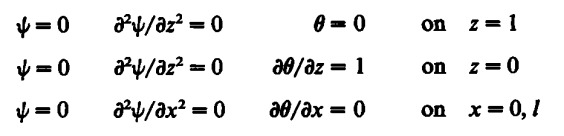
\includegraphics[width=8cm]{images/streamfunction/rimc81}} \hspace{0.5cm} 
\fbox{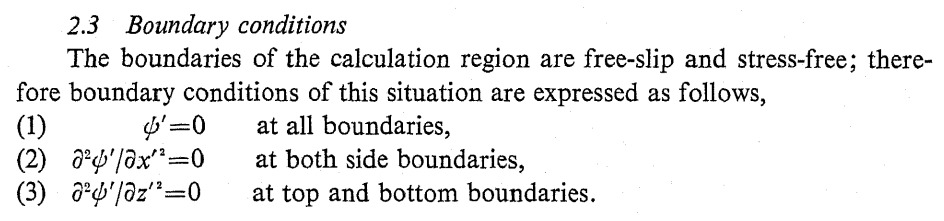
\includegraphics[width=8cm]{images/streamfunction/mato83}}\\
(`` free stress b.c.'') \textcite{rimc81} \hspace{3cm} \textcite{mato83} (1983)
\end{center}

\begin{center}
\fbox{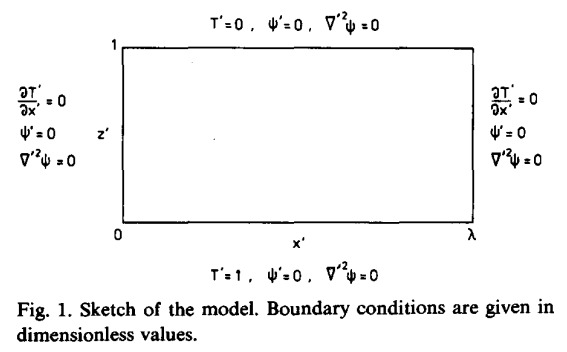
\includegraphics[width=7cm]{images/streamfunction/haeb84}}
\fbox{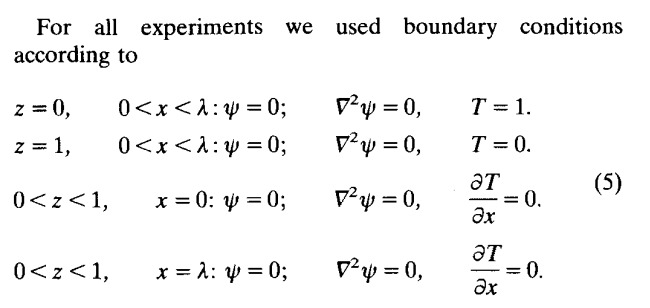
\includegraphics[width=7.8cm]{images/streamfunction/haeb88}}\\
\textcite{haeb84} \hspace{4cm} \textcite{haeb88}
\end{center}

\begin{center}
\fbox{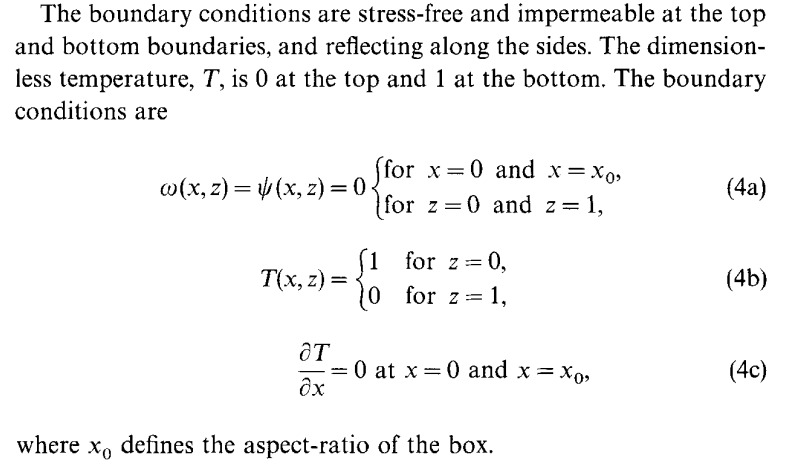
\includegraphics[width=7cm]{images/streamfunction/laym97}}\\
\textcite{laym97}
\end{center}

%------------------------
\subsection{No slip}

Rather counter intuitively no-slip boundary conditions prove to be substantially 
more difficult to implement than free-slip boundary conditions.
For example we find in \textcite{dedz03} (2003):
\begin{displayquote}
{\color{darkgray}
``According to \textcite{layt99} (1999), there are at least three natural ways of imposing zero tangential
velocities value along the boundary:
(i) Lagrange multiplier of tangential velocity component equal to zero as a constraint;
(ii) Penalty term imposing tangential velocity component equal to zero approximately;
(iii) Replacing no-slip with slip with friction.
''}
\end{displayquote}

Let us consider the bottom boundary. No-slip means $u=v=0$, i.e.
$\frac{\partial \Psi}{\partial y}=\frac{\partial \Psi}{\partial x}=0$. 
We have seen previously that $v=0$ yields $\Psi=$constant on the boundary,
leaving $\frac{\partial \Psi}{\partial y}=0$. This is problematic because if 
one solves the biharmonic equation as two Poisson equations for $\omega$ and $\Psi$
it does not translate to a boundary condition for $\omega$!

In general zeroing the tangential component of the velocity on a boundary will 
write $\partial \Psi/ \partial n =0$ where $n$ is the normal to the boundary.

\begin{center}
\fbox{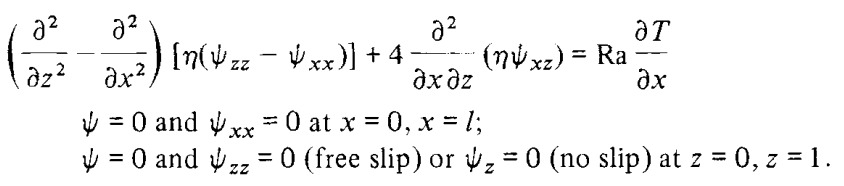
\includegraphics[height=2cm]{images/streamfunction/chri84}} 
\fbox{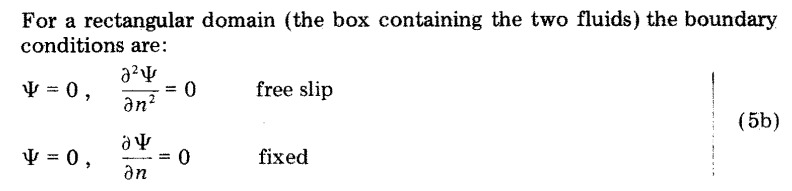
\includegraphics[height=2cm]{images/streamfunction/woid78}}\\
\textcite{chri84} (1984) \hspace{4cm}
\textcite{woid78} (1978)
\end{center}


Here $u$ is prescribed at the top, but not zero:
\begin{center}
\fbox{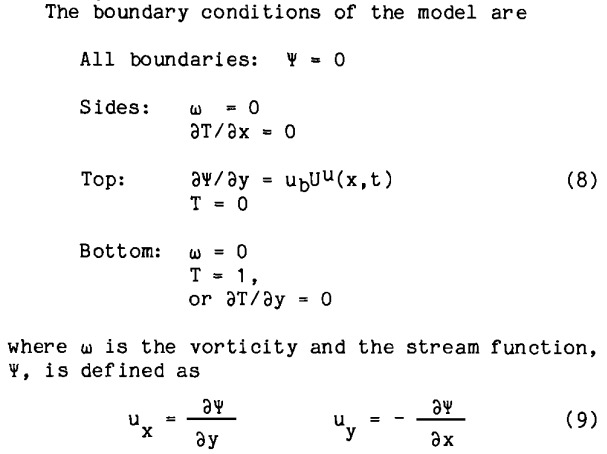
\includegraphics[width=7cm]{images/streamfunction/guda86c}}\\
\textcite{guda86c}
\end{center}

In \textcite{ludt79} (1979) we find this great summary of the problem 
and the sketch of its solution:
\begin{displayquote}
{\color{darkgray}
``The numerical methods we have used are well established and easy to apply. If we introduce
the vorticity $\omega$, then the fourth-order stream function equation can be
separated into a pair of second-order Poisson equations,
\[
\omega = -\vec\nabla^2 \Psi 
\qquad
\vec\nabla^2 \omega = -\frac{\partial T}{\partial x},
\]
for which efficient matrix reduction methods are available. 
For prescribed stress boundary conditions, the Poisson equations can simply
be solved successively as done by \textcite{mcrw74} (1974). 
A complication arises for a prescribed boundary velocity because the boundary conditions on vorticity are then not
explicit, see \textcite{rich73} (1973). On the boundary the vorticity is proportional to the shear stress
and, since the shear stress is not known until the flow field is found, we lack a boundary
condition on $\omega$. The Poisson equation for the stream function has an over-prescribed
boundary condition, since both $\Psi$, and $\partial\Psi/\partial y$ are given. 
This dilemma is resolved by using
the condition on $\Psi$ for the stream function equation and the condition on $\partial\Psi/\partial y$ in a
Taylor series expansion for $\omega$ at the boundary for the vorticity equation. To ensure
numerical stability with this boundary condition, it is necessary to iterate between the
equations; an efficient way of optimizing this iteration has been given by \textcite{ehgu75} (1975). The iteration technique for the coupled Poisson equations was tested against
analytical solutions of the biharmonic equation given by \textcite{davi77} (1977) 
and shown to be very accurate. The solution of the convection problem described here evolves 
with time, so the boundary condition on $\omega$ must be found at each time step by the iteration method.
This procedure is time consuming, so to increase the rate of convergence of this iteration a
boundary condition on $\omega$ accurate to first order (Taylor series) is used.''
}
\end{displayquote}

\noindent In \textcite{comn94} (1994) we read:
\begin{displayquote}
{\color{darkgray}
In the analysis of two-dimensional incompressible flows the streamfunction-vorticity formula-
tion of the Navier-Stokes equations allows the elimination of pressure from the problem and
automatically satisfies the continuity constraint. On the other hand, the value of the vorticity
at no-slip boundaries is difficult to specify and a poor evaluation of this boundary condition
leads, almost invariably, to serious difficulties in obtaining a converged solution.
[...] A guideline for a correct specification of boundary conditions at no-slip walls has been given
by Roache.' His numerical recipe can be summarized as follows: at no-slip wallsjirst specify the
streamfunction and then, in the procurement of the wall vorticity, utilize the additional information
on the normal component of the streamfunction. In this way the boundary conditions for the
streamfunction are not overspecified and the wall vorticity is correctly related to the tangential
component of the velocity. Obviously, at stationary walls the tangential component of the
velocity is zero, but at moving walls serious errors may result if the gradient of the streamfunction
is not properly taken into account.
}
\end{displayquote}


%------------------------------
\subsection{Stress b.c.}

{\color{orange} To Do}

%------------------------------
\subsection{Line of symmetry}

When the flow is truly symmetrical, the axis of symmetry can be considered a streamline. Therefore the
value of streamfunction along this boundary can be specified. Obviously, the velocity component normal
to the the symmetry boundary would be zero, whereas the streamwise component is extrapolated from
the interior solution.








%%%%%%%%%%%%%%%%%%%%%%%%%%%%%%%%%%%%%%%%%%%%%%%%%%%%%%%%%%%%%%%%%%%%%
\section{Pressure Poisson Equation for the isoviscous N-S equation}

This section is inspired by Salih.

The PPE can be derived by taking the divergence of vector form of momentum equation
\begin{equation}
\vec\nabla \cdot \left[ 
\frac{\partial \vec\upnu}{\partial t} + (\vec\upnu\cdot\vec\nabla) \vec\upnu \right] 
=
\vec\nabla \cdot \left[ - \frac{1}{\rho }\vec\nabla p +  \nu \vec\nabla^2 \vec\upnu  \right] 
\label{eq:sf10}
\end{equation}
or,
\begin{eqnarray}
\frac{\partial u}{\partial t}  + u \frac{\partial u}{\partial x}+ v \frac{\partial u}{\partial y}
&=& -\frac{1}{\rho} \frac{\partial p}{\partial x} 
+ \nu \left( \frac{\partial^2 u}{\partial x^2} + \frac{\partial^2 u}{\partial y^2} \right) \\
\frac{\partial v}{\partial t}  + u \frac{\partial v}{\partial x}+ v \frac{\partial v}{\partial y}
&=& -\frac{1}{\rho} \frac{\partial p}{\partial y} 
+ \nu \left( \frac{\partial^2 v}{\partial x^2} + \frac{\partial^2 v}{\partial y^2} \right) 
\end{eqnarray}
Differentiating these equations with respect to $x$ and $y$ respectively, and assuming $\rho$ constant in 
space yields
\begin{eqnarray}
\frac{\partial^2 u}{\partial x \partial t}  
+ \frac{\partial u}{\partial x} \frac{\partial u}{\partial x}+ u \frac{\partial^2 u}{\partial x^2}
+ \frac{\partial v}{\partial x} \frac{\partial u}{\partial y}+ v \frac{\partial^2 u}{\partial x\partial y}
&=& 
-\frac{1}{\rho} \frac{\partial^2 p}{\partial x^2} 
+ \nu \frac{\partial }{\partial x} \left( \frac{\partial^2 u}{\partial x^2} + \frac{\partial^2 u}{\partial y^2} \right) 
\\
\frac{\partial^2 v}{\partial y \partial t}  
+ \frac{\partial u}{\partial y} \frac{\partial v}{\partial x}+ u \frac{\partial^2 v}{\partial y\partial x}
+ \frac{\partial v}{\partial y} \frac{\partial v}{\partial y}+ v \frac{\partial^2 v}{\partial y^2}
&=& 
-\frac{1}{\rho} \frac{\partial^2 p}{\partial y^2} 
+ \nu \frac{\partial }{\partial y}  \left( \frac{\partial^2 v}{\partial x^2} + \frac{\partial^2 v}{\partial y^2} \right) 
\end{eqnarray}
Adding both equations together, i.e. taking the divergence of the first equation, yields
\begin{eqnarray}
&&\frac{\partial^2 u}{\partial x \partial t}  
+ \frac{\partial u}{\partial x} \frac{\partial u}{\partial x}+ u \frac{\partial^2 u}{\partial x^2}
+ \frac{\partial v}{\partial x} \frac{\partial u}{\partial y}+ v \frac{\partial^2 u}{\partial x\partial y}
\frac{\partial^2 v}{\partial y \partial t}  
+ \frac{\partial u}{\partial y} \frac{\partial v}{\partial x}+ u \frac{\partial^2 v}{\partial y\partial x}
+ \frac{\partial v}{\partial y} \frac{\partial v}{\partial y}+ v \frac{\partial^2 v}{\partial y^2} \\
&=&
-\frac{1}{\rho} \frac{\partial^2 p}{\partial x^2} 
+ \nu \frac{\partial }{\partial x} \left( \frac{\partial^2 u}{\partial x^2} + \frac{\partial^2 u}{\partial y^2} \right) 
-\frac{1}{\rho} \frac{\partial^2 p}{\partial y^2} 
+ \nu \frac{\partial }{\partial y}  \left( \frac{\partial^2 v}{\partial x^2} + \frac{\partial^2 v}{\partial y^2} \right) 
\end{eqnarray}

\begin{eqnarray}
&&\partial_t ( \underbrace{\frac{\partial u}{\partial x } +  \frac{\partial v}{\partial y } }_{=0}  )
+ \frac{\partial u}{\partial x} \frac{\partial u}{\partial x}
+ \frac{\partial u}{\partial y} \frac{\partial v}{\partial x}
+ \frac{\partial v}{\partial x} \frac{\partial u}{\partial y}
+ \frac{\partial v}{\partial y} \frac{\partial v}{\partial y}
+ u (\underbrace{\frac{\partial^2 u}{\partial x^2} +  \frac{\partial^2 v}{\partial y\partial x}}_{A} )
+ v (\underbrace{\frac{\partial^2 v}{\partial y^2} +  \frac{\partial^2 u}{\partial x\partial y}}_{B} )\\
&=&
-\frac{1}{\rho} (\frac{\partial^2 p}{\partial x^2} + \frac{\partial^2 p}{\partial y^2})
+ \nu \frac{\partial }{\partial x} \left( \frac{\partial^2 u}{\partial x^2} + \frac{\partial^2 u}{\partial y^2} \right) 
+ \nu \frac{\partial }{\partial y}  \left( \frac{\partial^2 v}{\partial x^2} + \frac{\partial^2 v}{\partial y^2} \right) 
\end{eqnarray}


We have
\[
A = 
\frac{\partial^2 u}{\partial x^2} +  \frac{\partial^2 v}{\partial y\partial x}
=\frac{\partial u}{\partial x} ( \frac{\partial u}{\partial x}+ \frac{\partial v}{\partial y}) = 0
\]
\[
B 
=\frac{\partial^2 v}{\partial y^2}  +  \frac{\partial^2 u}{\partial x\partial y}
=\frac{\partial v}{\partial y} (\frac{\partial u}{\partial x} + \frac{\partial v}{\partial y}) =0
\]
so that 
\begin{eqnarray}
(\frac{\partial u}{\partial x})^2 
+ 2\frac{\partial u}{\partial y} \frac{\partial v}{\partial x}
+ (\frac{\partial v}{\partial y} )^2
=
-\frac{1}{\rho} (\frac{\partial^2 p}{\partial x^2} + \frac{\partial^2 p}{\partial y^2})
+ \nu \frac{\partial }{\partial x} \left( \frac{\partial^2 u}{\partial x^2} + \frac{\partial^2 u}{\partial y^2} \right) 
+ \nu \frac{\partial }{\partial y}  \left( \frac{\partial^2 v}{\partial x^2} + \frac{\partial^2 v}{\partial y^2} \right) 
\end{eqnarray}



The viscosity terms in the rhs can be rearranged as
\[
\frac{\partial }{\partial x} \left( \frac{\partial^2 u}{\partial x^2} + \frac{\partial^2 u}{\partial y^2} \right)
+ \frac{\partial }{\partial y}  \left( \frac{\partial^2 v}{\partial x^2} + \frac{\partial^2 v}{\partial y^2} \right)
=
\frac{\partial^2 }{\partial x^2} (\frac{\partial u}{\partial x} +\frac{\partial v}{\partial y} ) 
+
\frac{\partial^2 }{\partial y^2} (\frac{\partial u}{\partial x} +\frac{\partial v}{\partial y} )
=0
\]
We are left with
\begin{eqnarray}
(\frac{\partial u}{\partial x})^2 
+ 2\frac{\partial u}{\partial y} \frac{\partial v}{\partial x}
+ (\frac{\partial v}{\partial y} )^2
=
-\frac{1}{\rho} (\frac{\partial^2 p}{\partial x^2} + \frac{\partial^2 p}{\partial y^2})
\end{eqnarray}
Now, the left-hand side can be further reduced as follows
\[
(\frac{\partial u}{\partial x})^2 
+ 2\frac{\partial u}{\partial y} \frac{\partial v}{\partial x}
+ (\frac{\partial v}{\partial y} )^2
= ( \underbrace{\frac{\partial u}{\partial x}+ \frac{\partial v}{\partial y} }_{=0})^2
- 2 \frac{\partial u}{\partial x} \frac{\partial v}{\partial y}
+ 2\frac{\partial u}{\partial y} \frac{\partial v}{\partial x}
\]
In the end
\[
\vec\nabla^2 p = 2\rho  \left(
\frac{\partial u}{\partial x}\frac{\partial v}{\partial y}-
\frac{\partial v}{\partial x}\frac{\partial u}{\partial y}
\right)
\]
The PPE can also be written in terns of stream function:
\[
\boxed{
\vec\nabla^2 p = 2\rho  \left[
\frac{\partial^2 \Psi}{\partial x^2}\frac{\partial^2 \Psi}{\partial y^2}-
\left(\frac{\partial^2 \Psi}{\partial x \partial y}\right)^2
\right]
}
\]
The Poisson equation for pressure is an elliptic equation, showing the elliptic nature of pressure in incompressible flows. For a steady flow problem, the PPE is solved only once, i.e., after the steady state
values of $\omega$ and $\Psi$ have been computed.

Having established the PDE we must now turn to the boundary conditions. 
On a solid boundary, boundary values of pressure are obtained using the tangential momentum equation 
of the fluid adjacent to the wall surface. For a wall located at $y=0$ in Cartesian coordinate system (i.e.
the bottom boundary), the tangential momentum equation, that is  the $x$-momentum equation, reduces to
\[
\left.\frac{\partial p}{\partial x}\right\rvert_{wall} 
= \eta \left.\frac{\partial^2 u}{\partial y^2}\right\rvert_{wall}
= -\eta \left. \frac{\partial \omega}{\partial y}\right\rvert_{wall}
\]
since $v= \partial_x v =0$ on that boundary.

\vspace{1cm}

In \textcite{reddybook2} we find at page 163:  The pressure, if required, may be computed from a Poisson equation of the form:
\[
\Delta P = \vec\nabla \cdot(\vec{f} - \nu \Delta \vec\upnu - (\vec\upnu\cdot\vec\nabla) \vec\upnu)
\]








%%%%%%%%%%%%%%%%%%%%%%%%%%%%%%%%%%%%%%%%%%%%%%%%%%%%%%%%%%
\section{Vorticity-stream function formulation in 3D}

The vorticity-streamfunction approach has seen considerable use for two-dimensional incompressible flows. It has become less popular in recent years because its extension to three-dimensional flows is difficult.
Both the vorticity and streamfunction become three-component vectors in three dimensions
so one has a system of six partial differential equations in place of the four that are necessary in a velocity-pressure formulation. It also inherits the difficulties in dealing with variable fluid properties, compressibility, and boundary conditions that were described above for two dimensional flows.

In \textcite{reddybook2} we find at page 163: 
\begin{displayquote}
{\color{darkgray}
``
A 3D version of the  vorticiy transport equation is possible, 
although it has seen relatively little use in computation due to the complexity 
of the vorticity boundary conditions.
'' }
\end{displayquote}

\noindent \textcite{glte87} (1987) state: ``
\begin{displayquote}
{\color{darkgray}
The extension of the codes to three dimensions is not easy
for the vorticity stream-function formulation. In three dimensions, the vorticity-
stretching term does not vanish and the equation system has two nonlinear terms.
''}
\end{displayquote}



\noindent In \textcite{zhym12} (2012) we read:
\begin{displayquote}
{\color{darkgray}
``For 3-D mantle convection, we can likewise employ the
poloidal potential $\Phi$ and a vorticity-like scalar function $\Omega$
(Busse, 1989; Chandrasekhar, 1961; Travis et al., 1990). It is
to be noted that this potential $\Phi$ is not the same as the stream
function $\Psi$ in 2-D (see Chapter 7.04). From the general representation 
of an arbitrary solenoidal vector field (Busse, 1989),
we can write a 3-D velocity vector as
\[
\vec\upnu = \vec\nabla \times \vec\nabla \times (\Phi \vec{e}_z) + \vec\nabla \times (\Theta \vec{e}_z)  
\]
where $\vec{e}_z$ is the unit vector in the vertical, $z$-direction, pointing upward.
$\Theta$ is the toroidal potential and is present in problems
with lateral variations of viscosity (Christensen and Harder,
1991; Gable et al., 1991; Zhang and Christensen, 1993).
Thus, for constant viscosity, $\Theta$ is zero unless driven by a
boundary condition (e.g., Gable et al., 1991), and the velocity
vector $\vec\upnu=(u,v,w)$ involves higher-order derivatives of $\Phi$ in this
formulation:
\[
u = \frac{\partial^2 \Phi}{\partial y\partial z}
\qquad
v = \frac{\partial^2 \Phi}{\partial x \partial z}
\qquad
w = - (\frac{\partial^2 \Phi}{\partial x^2} + \frac{\partial^2 \Phi}{\partial y^2})
\]
The 3-D momentum equation for constant properties can
be written as a system of coupled Poisson equations in 3-D:
\begin{eqnarray}
\vec\nabla^2 \Phi &=& \Omega \\
\vec\nabla^2 \Omega &=& \Ranb T
\end{eqnarray}
where all differential operators are 3-D in character and $\Omega$ is a
scalar function playing a role analogous to the vorticity in the
2-D formulation.

We note that FD and FV methods using the primitive variables 
of velocity and pressure are currently predominant in
models of 3-D mantle convection with variable viscosity.
''}
\end{displayquote}


\vspace{0.5cm}




{\color{orange}
ToDo:
\begin{enumerate}
\item scan 3D literature 
\item find all formulations cartesian or not
\item document num methods used
\end{enumerate}
}

%...................................
\subsection{Cartesian domain (1)}
\textcite{sola99} (1999) write:
\begin{displayquote}
{\color{darkgray}
``
The conservation equations for momentum and mass are transformed into four Poisson equations by introducing a vector potential stream function $\Psi$ and vorticity $\omega$ \cite{tros90}:
\begin{eqnarray}
\Delta \Psi_x  + \omega_x &=& 0 \\
\Delta \omega_x - \Ranb_T \frac{\partial T}{\partial y} &=& 0 \\
\Delta \Psi_y  + \omega_y &=& 0 \\
\Delta \omega_y + \Ranb_T \frac{\partial T}{\partial x} &=& 0 
\end{eqnarray}
Since the buoyancy force acts only in the $z$-direction, $\Psi_z$ and 
$\omega_z$ vanish identically. Shear-stress free boundaries on top and bottom
yields the following boundary conditions:
\[
\omega_x=\omega_y = \Psi_x=\Psi_y=0 
\]
at the top and bottom. Periodicity is assumed on all vertical boundaries.

The four Poisson equations are solved using a multigrid iterative
method described by \textcite{past94} (1994) and Sotin et al. 1995.
''}
\end{displayquote}

%---------------------------------
\subsection{Cartesian domain (2)}

Let us now turn to \textcite{laym96} (1996): 
\begin{displayquote}
{\color{darkgray}
``For the spatial discretization fourth-order correct bi-cubic splines are employed \cite{mayu91}. [...] The mesh is uniform in the horizontal direction, and non-uniform
in the vertical direction with mesh-refinement near the boundary layers. [...]
The mechanical boundary conditions are stress-free and
impermeable at the top and bottom boundaries,
and reflecting along the sides. The dimensionless
temperature $T$ is zero at the top and unity at the
bottom ($z = 1$), and there is zero heat flux along the sides.''
}
\end{displayquote}

\noindent In \textcite{laym97} (1997) the authors start with a 2D formulation:
\begin{displayquote}
{\color{darkgray}
``Instead of the biharmonic equation for $\Psi$, (e.g., \textcite{chri84}, 1984), the conservation equations for the mass and momentum are given by two 
second-order partial differential equations (1) and (2). The horizontal and vertical coordinates are, respectively, x and z with z pointing upwards. Time, $t$, has been
non-dimensionalized by the thermal diffusion time across the depth of
the layer. A more detailed description of the scheme for non-dimensionalization is given in \textcite{weoy89} (1989).
The boundary conditions are stress-free and impermeable at the top
and bottom boundaries, and reflecting along the sides. The dimension-
less temperature, T, is 0 at the top and 1 at the bottom. The boundary
conditions are: $\Psi=\omega=0$ on all sides.''
}
\end{displayquote}
They go further and explain the 3D approach:
\begin{displayquote}
{\color{darkgray}
``
We employ the poloidal potential, $\Psi$, and a vorticity-like scalar function 
$\Omega$ for solving the momentum equation with constant properties
(\textcite{buss89}, 1989; \textcite{tros90}, 1990b). 
We note that the potential $\Psi$ is not
the same as the streamfunction in two dimensions. From the general
representation of an arbitrary solenoidal vector field (\textcite{buss89}, 1989), we
can write a three-dimensional velocity vector,
\[
\vec\upnu = \vec\nabla \times ( \vec\nabla \times \vec{e}_z\Psi  )
\]
with the $\vec{e}_z$ axis pointing upwards. Thus the velocity vector involves
higher-order derivatives of in this formulation:
\[
u=\frac{\partial^2 \Psi}{\partial x\partial z}
\qquad
v=\frac{\partial^2 \Psi}{\partial y\partial z}
\qquad
\omega = -
\left(
\frac{\partial^2\Psi }{\partial x^2}
+\frac{\partial^2\Psi }{\partial y^2}
\right)
\]
with $\vec\upnu=(u, v, w)$. The three-dimensional momentum equation can be
written as a system of coupled Poisson equations:
\[
\vec\nabla^2 \Psi = \Omega  
\qquad
\vec\nabla^2 \Omega = \Ranb T 
\]
Here $\Omega$ is a scalar function playing an analogous role to the vorticity
in the two-dimensional formulation.

The numerical method employed in this paper is based on a recursive
algorithm for generating the weights in the finite-difference approximation.''}
\end{displayquote}

%-----------------------------------
\subsection{Cartesian domain (3)}

See for example \textcite{hous90} (1990) and refs therein:
\begin{displayquote}
{\color{darkgray}
``As the flow is incompressible, velocity may
be expressed as the curl of a solenoidal vector potential $\vec\Psi$
[e.g. Richardson \& Cornish (1977)]:
\[
\vec \upnu = \vec\nabla \times \vec\Psi
\]
For 2-D flow, 3 is a vector everywhere normal to the plane
of the flow. It may then be treated as a scalar, and is given
the name streamfunction.

The momentum equation may be restated as a biharmonic equation:
\[
\vec\nabla^4 \vec\Psi = \vec{f}
\]
where $\vec{f}$ is minus the curl of the buoyancy force divided by
viscosity, and is hereafter treated as a known quantity. It is
also useful to define the vorticity, which is simply related to
the potential function
\[
\vec\omega = \vec\nabla \times \vec\upnu = -\vec\nabla^2 \Psi
\]
We now consider a finite difference technique for solving
equation (3) in a region spanned by a regular isotropic array
of nodes.'' }
\end{displayquote}

Boundary conditions of all kinds are extensively discussed!


%................................
\subsection{Spherical shell}

\textcite{zess80} (1980) present axisymmetric steady convective solutions

Likewise \textcite{sope90,sope94}: ``The model is
spherical but restricted in generality to the analysis of axisymmetric solutions.''



%%%%%%%%%%%%%%%%%%%%%%%%%%%%%%%%%%%%%%%%%%%%%%%%%%%%%%%%%%%%%%%%%%%%%%%%%%%%%%%%%%
\section{Vorticity-stream function formulation in polar/cylindrical coordinates}

\url{https://en.wikipedia.org/wiki/Stokes_stream_function} uses very different 
definitions! {\color{orange} sort it out!} 
actually it is for three-dimensional incompressible flow with axisymmetry!

\[
\upnu_r=\frac{1}{r}\frac{\partial \Psi}{\partial \theta} 
\]
\[
\upnu_\theta=-\frac{\partial \Psi}{\partial r} 
\]
\[
\vec \omega
=
\left( \frac{1}{r} \frac{\partial \upnu_z}{\partial \theta} -\frac{\partial \upnu_\theta}{\partial z}  \right) \vec{e}_r +
\left(  \frac{\partial \upnu_r}{\partial z}-\frac{\partial \upnu_z}{\partial r} \right) \vec{e}_\theta +
\left( \frac{1}{r}\frac{\partial (r \upnu_\theta)}{\partial r}-\frac{1}{r}\frac{\partial \upnu_r}{\partial \theta}  \right) \vec{e}_z 
\]

\[
\vec\nabla^4 \Psi= 
\left(
\frac{\partial^2}{\partial r^2}
+\frac{1}{r}\frac{\partial }{\partial r}
+\frac{1}{r^2}\frac{\partial^2 }{\partial \theta^2}
\right)
\left(
\frac{\partial^2 \Psi}{\partial r^2}
+\frac{1}{r}\frac{\partial \Psi}{\partial r}
+\frac{1}{r^2}\frac{\partial^2 \Psi}{\partial \theta^2}
\right)
\]
or
\[
\vec\nabla^4 \Psi= 
\Psi_{,rrrr}
+\frac{2}{r}\Psi_{,rrr}
-\frac{1}{r^2}(\Psi_{,rr}-2\Psi_{,rr\theta\theta})
+\frac{1}{r^3}(\Psi_{,r} -2\Psi_{,r\theta\theta})
+\frac{1}{r^4}(4\Psi_{,\theta\theta}+2\Psi_{,\theta\theta\theta\theta})
\]

See \textcite{hsui78}. \cite{tosl78} \cite{trol94}

%%%%%%%%%%%%%%%%%%%%%%%%%%%%%%%%%%%%%%%%%%%%%%%%%%%%%%%%%%%%%%%%%%%%%%%%%%%%%%%%%%
\section{Vorticity-stream function formulation in spherical coordinates
for three-dimensional incompressible flow with axisymmetry}

What follows comes from \url{https://en.wikipedia.org/wiki/Stokes_stream_function}.

The flow velocity components $\upnu_r$ and $\upnu_\theta$ 
are related to the Stokes stream function $\Psi$ through:
\[
\upnu_r = \frac{1}{r^2 \sin \theta} \frac{\partial \Psi}{\partial \theta}
\qquad
\upnu_\theta = -\frac{1}{r \sin \theta} \frac{\partial \Psi}{\partial r}
\]
The azimuthal velocity component $\upnu_\phi$ is not a function of the Stokes stream function $\Psi$.

\begin{center}
\includegraphics[width=3cm]{images/sphcoord}
\end{center}

The vorticity is defined as:
\[
\vec\omega = \vec\nabla \times \vec\upnu = \vec\nabla\times\vec\nabla\times \psi
\qquad
{\text with}
\qquad
\psi = -\frac{\Psi}{r \sin \theta} \vec{e}_\phi
\]
From the definition of the curl in spherical coordinates\footnote{\url{https://en.wikipedia.org/wiki/Del_in_cylindrical_and_spherical_coordinates}}:
\begin{eqnarray}
\omega_r &=& \frac{1}{r \sin\theta} \left( \frac{\partial}{\partial \theta}
(\upnu_\phi \sin\theta) - \frac{\partial \upnu_\theta}{\partial \phi}\right) \vec{e}_r \\
\omega_\theta &=& \frac{1}{r} \left( \frac{1}{\sin\theta} 
\frac{\partial \upnu_r}{\partial \phi} - \frac{\partial}{\partial r}
(r \upnu_\phi)  \right) \vec{e}_\theta \\
\omega_\phi &=& \frac{1}{r} \left( 
\frac{\partial}{\partial r} (r \upnu_\theta) - \frac{\partial \upnu_r}{\partial \theta}\right) \vec{e}_\phi 
\end{eqnarray}
First notice that the $r$ and $\theta$ components are equal to $0$. {\color{orange} prove!}
Secondly substitute $\upnu_r$ and $\upnu_\theta$ into $\omega_\phi$.
The result is:
\begin{eqnarray}
\omega_r &=& 0 \\
\omega_\theta &=& 0 \\
\omega_\phi &=& \frac{1}{r}
\left[
\frac{\partial }{\partial r} \left(r \left( -\frac{1}{r \sin \theta} \frac{\partial \Psi}{\partial r}
\right)\right) - \frac{\partial}{\partial \theta} \left( \frac{1}{r^2 \sin\theta} \frac{\partial \Psi}{\partial \theta}  \right)
\right]
\end{eqnarray}
After some algebra we arrive at
\[
\vec\omega
= 
\left(
\begin{array}{c}
0 \\ 0 \\
-\frac{1}{r \sin\theta} \left(  \frac{\partial^2 \Psi}{\partial r^2} 
+ \frac{\sin\theta}{r^2} \frac{\partial}{\partial \theta}
\left(
\frac{1}{\sin \theta} \frac{\partial \Psi}{\partial \theta}
\right)
\right)
\end{array}
\right)
\]

Proof that velocity is perpendicular to gradient of stream function:
\[
\vec\nabla \Psi \cdot \vec\upnu 
= \frac{\partial \Psi}{\partial r} \cdot \frac{1}{r^2 \sin\theta} \frac{\partial \Psi}{\partial \theta}
+ \frac{1}{r} \frac{\partial \Psi}{\partial \theta} \cdot
\left( 
-\frac{1}{r \sin\theta} \frac{\partial \Psi}{\partial r}
\right) 
=0
\]


%%%%%%%%%%%%%%%%%%%%%%%%%%%%%%%%%%%%%%%%%%%%%%%%%%%%%%%%%%%%%%%%
\section{Numerical approach}

When it comes to solving the biharmonic equation, there are essentially two options:
solving/discretising the biharmonic operator involving 4th order derivatives, 
or introducing the vorticity and solving coupled PDEs in vorticity-stream function.

\textcite{mayu92} state: 
\begin{displayquote}
{\color{darkgray}
`` The fourth-order elliptic equation does not contain time explicitly. One can
obtain the stream-function for a given temperature field by solving this nonlinear
equation at each instant. Equation (12) is a nonlinear time-dependent advection-
diffusion equation, where the $\Psi(T)$ dependence is given by the biharmonic eq. Numerical solution
of the advection-diffusion equation with advection dominating over diffusion is fraught
with numerical difficulties. It is known that high-order finite-element and finite-
difference schemes deteriorate from errors located near steep gradients of the advected
field. Various upwinding schemes, designed to overcome this difficulty, introduce
artificial smoothing (Cuvelier et al., 1988). A finite-element scheme based on the
Lagrangian formulation of the total time derivative in the advection-diffusion equation
\cite{mayu91} proves to be very efficient for the high Rayleigh number
Newtonian convection. In stress-softening fluid, thermal advection can be very strong
locally due to the decrease of the effective viscosity with growing stress. Therefore,
we have chosen the Lagrangian scheme to solve the energy equation for the
non-Newtonian case. A second-order predictor-corrector scheme with Lagrangian
formulation was applied for time-stepping in the energy equation. The Lagrangian scheme requires
interpolation to compute values of $\Psi$ and $T$ between nodal points. This scheme is
very sensitive to the quality of spatial approximation. We used bicubic splines (Ahlberg
et al., 1967) for spatial discretization of both the temperature and stream-function.
''}
\end{displayquote}

\noindent Rather interestingly \textcite{popo92} (1992) state: 
\begin{displayquote}
{\color{darkgray}
``
There is a class of methods based on the introduction of a
stream function which satisfies this condition automatically
and gives good results. However, the stress-free boundary
condition causes significant difficulties because it requires
the calculation of third-order derivatives of the stream
function. These algorithms are also not applicable for
irregular meshes. Thus, it is difficult to solve problems in
regions with complicated geometry, and to refine the mesh
in areas of special interest. A further disadvantage is that
the approximation functions are not expressed explicitly in
terms of the nodal variables and an additional system of
linear equations must be solved.
'' }
\end{displayquote}

%--------------------------------
\subsection{Finite differences}

In \textcite{vanv08} we find 
\begin{displayquote}
{\color{darkgray}
``To solve the equation of motion we have applied a second-order, central finite-
difference scheme. We considered free slip (zero shear stress) boundary conditions at all
boundaries. The solution of the equation on each node was then computed in
terms of the 12 nearest nodes. The system matrix was square, symmetric and diagonally
dominant, with only 12 non-null diagonals. This system could be solved by a very robust
method based on a LU triangular factorization by Gaussian elimination with partial
pivoting, which is already implemented in the standard MATLAB code.''
}
\end{displayquote}


\noindent In \textcite{zhym12} (2012) we read:
\begin{displayquote}
{\color{darkgray}
``We note that solving the biharmonic equation by FDs takes more time than 
solving two coupled Laplacian equations.''
}
\end{displayquote}


\vspace{1cm}

{\color{orange}
ToDo:
\begin{enumerate}
\item scan literature. e.g. \textcite{mcrw74} (1974) explain their stencils
\item establish stencil(s) for equations
\item how to deal with boundaries
\item In gerya's book it is solved with FD. see page 72, and example Streamfunction2D.m - translate to python?
\end{enumerate}
}

%--------------------------------
\subsection{Finite elements}

We start from $\vec\nabla^2 \vec\nabla^2 \Psi = f$, which we rewrite as follows:
\begin{eqnarray}
\vec\nabla^2 \Psi &=& -\omega \\
\vec\nabla^2 \omega &=& f
\end{eqnarray}
After establishing the weak form and discretising it, this will yield the following linear system:
\[
\left(
\begin{array}{cc}
K & M \\
0 & K
\end{array}
\right)
\cdot
\left(
\begin{array}{cc}
\vec\Psi\\
\vec\omega
\end{array}
\right)
=
\left(
\begin{array}{cc}
\vec 0\\
\vec f
\end{array}
\right)
\]
where $K=\int B^T B dV$. 
This is an ideal situation: one can first solve the second line, obtain $\vec\omega$
and then solve the first line as $K \cdot \vec \Psi = - M \cdot \vec\omega$
Also it is the same matrix $K$, only different rhs!

{\color{teal} Can i do this with Q1 elements only?!}

Remarks:

\begin{itemize}
\item 
See \textcite{grsa} p523-525 for important remarks about establishing the weak forms of the vorticity-stream function equations. They refer to \cite{stev82}.

\item 
In Step~47 of deal.II\footnote{\url{https://www.dealii.org/current/doxygen/deal.II/step_47.html}} it is explained 
\begin{displayquote}
{\color{darkgray}
``The fundamental issue with the equation is that [the biharmonic equation] takes four 
derivatives of the solution. In the case of the Laplace equation [...], and several other 
tutorial programs, one multiplies by a test function, integrates, integrates by parts, 
and ends up with only one derivative on both the test function and trial function - 
something one can do with functions that are continuous globally, but may have kinks 
at the interfaces between cells: The derivative may not be defined at the interfaces, 
but that is on a lower-dimensional manifold (and so doesn't show up in the integrated value).\\
But for the biharmonic equation, if one followed the same procedure using integrals over 
the entire domain (i.e., the union of all cells), one would end up with two derivatives 
on the test functions and trial functions each. If one were to use the usual piecewise 
polynomial functions with their kinks on cell interfaces, the first derivative would 
yield a discontinuous gradient, and the second derivative with delta functions on the 
interfaces - but because both the second derivatives of the test functions and of the 
trial functions yield a delta function, we would try to integrate the product of two delta functions.''}
\end{displayquote}
Logically the biharmonic equation is then split into two Poisson equations.

\item In van Keken's phd thesis we read: 
\begin{displayquote}
{\color{darkgray}
``The equation of motion is a 4th-order PDE and, 
for a FE approximation to be conform, the basis functions should be twice 
continuously differentiable in each element and least continuously differentiable throughout
the computational domain $\Omega$. ''
}
\end{displayquote}
van Keken then proceeds to use 2 different methods: a non-conforming type of element
\textcite{haeb84} (1984), and a bicubic spline FE method \textcite{woid78} (1978), \textcite{kopi79} (1979).

\item check \textcite{comn94} (1994) for N-S implementation.

\end{itemize}

%........................................
\subsubsection{the Spline FE method} 

\textcite{chri84} (1984) writes:
\begin{displayquote}
{\color{darkgray}
``The numerical grid consists of rectangular elements of variable size. All spatially varying quantities - i.e. $\Psi$, $T$ and $\eta$ are represented by polynomial splines. These are polynomials of a certain degree $n$ within each individual element which are continuous at the joints up to the $k$th derivative ( $k<n$). 
In a spline space at a rather compact base can be constructed,
which means that each base function (B spline) is zero outside a small region consisting of few elements; this is an advantage over a polynomial or Fourier space. 
The shape of each B spline depends on the local grid structure. With the restriction that the size of the elements varies in both dimensions only by one of the factors 
$1/\alpha$, $1$ or $\alpha$ compared to the neighbouring elements (with $\alpha$ fixed) a restricted number of types of B splines are necessary which
reduces the computational costs. Splines which are non-zero at the boundary of the mathematical domain are modified in such a way that the boundary conditions to [the biharmonic equation] are fulfilled for any function that can be constructed in the spline space. Compared to the
normal finite element method with Lagrangian shape functions, higher requirements on the
continuity can be easily fulfilled. On the other hand one is restricted to semi-regular grids with all element boundaries parallel or perpendicular to each other.
[...]
The integral contains fourth-order derivatives, however, by partial integration it can be transformed into one containing only second derivatives. The matrix built is band
structured and a stable solution is obtained by a Cholesky transformation.''
}
\end{displayquote}

\noindent \textcite{chyu89} (1989) states: 
\begin{displayquote}
{\color{darkgray}
``The spline finite element method used to solve the set of
equations (7) and (9) is described by Christensen
[1984]. Bicubic splines are taken for $\Psi$,and biquadratic splines for $T$. The
grid is nonuniform and allows higher resolution in the boundary layers''
}
\end{displayquote}

\noindent In \textcite{mayu92} we find: 
\begin{displayquote}
{\color{darkgray}
``We can use the Galerkin method to approximate the solution. In this
case a matrix ${\bm A}$ is obtained as
\[
a_{ij} = \iint \eta
\left[
\left(\frac{\partial^2 B_i}{\partial y^2}-\frac{\partial^2 B_i}{\partial x^2}\right)
\left(\frac{\partial^2 B_j}{\partial y^2}-\frac{\partial^2 B_j}{\partial x^2}\right)
+4\frac{\partial B_i}{\partial y\partial x}\frac{\partial B_j}{\partial y \partial x}
\right]
dxdy
\]
where $B$ is a basic bicubic spline.
The derivatives of a basic spline (a piecewise cubic
polynomial) can be calculated analytically.''
}
\end{displayquote}

\vspace{0.5cm}

{\color{orange} 
ToDo: 
\begin{itemize}
\item derive B spline equation, implement, python fct? check for example \cite{kopi79}
\item derive equation above
\item work out the 2 formulations of vKK phd thesis
\end{itemize}
}

%%%%%%%%%%%%%%%%%%%%%%%%%%%%%%%%%%%%%%%%%%%%%%%%%%%%%%%%%%%%%
\section{Algorithm for stream function-vorticity formulation}

A solution algorithm for computing evolution of incompressible, two-dimensional flow using stream function-vorticity formulation is given as follows:
\begin{enumerate}
\item Initialize the velocity field and compute the associated vorticity field and streamfunction field
using equations $\omega_z = \partial_x v- \partial_y u$ and $\Delta \Psi = -\omega$.
\item Compute the boundary conditions for vorticity.
\item Solve the vorticity transport equation \eqref{eq:s22} to compute the vorticity at new time step; any standard time marching scheme may be used for this purpose.
\item Solve the Poisson equation for streamfunction $\Delta \Psi = -\omega$ to compute the streamfunction field at new time step; any iterative scheme for elliptic equations may be used.
\item Compute the velocity field at new time step using the relations $u=\partial_y \Psi$ and $v=-\partial_x \Psi$.
\item Return to step 2 and repeat the computation for another time step.
\end{enumerate}












%%%%%%%%%%%%%%%%%%%%%%%%%%%%%%%%%%%%%%%
\section{The nondimensional equations}

For the isoviscous case, and omitting the primes:
\[
\vec\nabla^4 \Psi = Ra \frac{\partial T}{\partial x}
\]

The vorticity equation is
\[
\frac{\partial \omega}{\partial t} +\vec\upnu \cdot \vec\nabla \omega =
Re^{-1} \vec\nabla^2 \omega
\]




\vspace{0.5cm}

{\color{orange} 
ToDo: 
\begin{itemize}
\item re-derive these equations , see for example \textcite{sope94} (1994) eq 8, 
or \textcite{kopi79} eq 1,2
\end{itemize}
}

%%%%%%%%%%%%%%%%%%%%%%%%%%%%%%%%%%%%%%%%%%%%%%
\section{Incorporation of phase changes}

\vspace{0.5cm}

{\color{orange} 
ToDo: 
\begin{itemize}
\item scan literature for $\Gamma$ fct
\item isolate example
\end{itemize}
}



%%%%%%%%%%%%%%%%%%%%%%%%%%%%%%%%%%%
\section{The energy equation}

The (simple) energy equation
\[
\frac{\partial T}{\partial t} + \vec\upnu \cdot \vec\nabla T = \kappa \Delta T
\]
becomes in 2D:
\[
\frac{\partial T}{\partial t} + 
\frac{\partial \Psi}{\partial y}\frac{\partial T}{\partial x} 
-\frac{\partial \Psi}{\partial x}\frac{\partial T}{\partial y} 
= \kappa \Delta T
\]

{\color{teal} rewrite with all coeffs}


%%%%%%%%%%%%%%%%%%%%%%%%
\section{Remark, misc}

Arie van den Berg (prov. comm.) writes:
\begin{displayquote}
{\color{darkgray}
``The stream function formulation is useful to obtain a conceptually
simpler implementation with finite differences if you rewrite the 4th
order biharmonic equation for the streamfunction in two coupled Poisson
equations for streamfunction and vorticity respectively. That is for an
isoviscous fluid. For variable viscosity it becomes more ugly.

It disappeared probably due its limitations for variable viscosity fluids
and once the more power full  but complex formulation alternatives
became more well known. ''
}
\end{displayquote}

In \textcite{grsa} (p.~941), the authors present an algorithm to compute $\Psi$
from a velocity field obtained via the FEM. 


















%-----------------------------------------------------------------------
\section{Literature}
%systematically already done 
%1970,1971,1972,1973,1974,1975,1976,1977,1978,1979
%1980,1981,1982,1983,1984,1985,1986,1987,1988,1989
%1990,1991,1992,1993,1994


\begin{scriptsize}
\begin{itemize}
\item[\nineteensixtyseven]
 \textbullet \fullcite{tuox67}
\item[\nineteensixtynine]
 \textbullet \fullcite{scto69}
\item[\nineteenseventy]
 \textbullet \fullcite{ramb70}
\item[\nineteenseventyone]
 \textbullet \fullcite{totu71b}\\
 \textbullet \fullcite{totu71}
\item[\nineteenseventythree]
 \textbullet \fullcite{rich73b}\\
 \textbullet \fullcite{rich73}\\
 \textbullet \fullcite{mcrw73}
\item[\nineteenseventyfour]
 \textbullet \fullcite{care74}\\
 \textbullet \fullcite{mcrw74}
\item[\nineteenseventyfive]
 \textbullet \fullcite{hemw75} \\
 \textbullet \fullcite{patt75}
\item[\nineteenseventysix]
 \textbullet \fullcite{patt76}
\item[\nineteenseventyseven]
 \textbullet \fullcite{davi77b} \\
 \textbullet \fullcite{davi77}
\item[\nineteenseventyeight]
 \textbullet \fullcite{bird78b} \\
 \textbullet \fullcite{hsui78} \\
 \textbullet \fullcite{gart78} \\
 \textbullet \fullcite{tosl78} \\
 \textbullet \fullcite{woid78} \\
 \textbullet \fullcite{rimc78}
\item[\nineteenseventynine]
 \textbullet \fullcite{grif79} \\
 \textbullet \fullcite{mcke79} \\
 \textbullet \fullcite{bobo79} \\
 \textbullet \fullcite{kopi79} \\
 \textbullet \fullcite{ludt79}
\item[\nineteeneighty]
 \textbullet \fullcite{jamc80} \\
 \textbullet \fullcite{zess80} \\
 \textbullet \fullcite{yupe80}
\item[\nineteeneightyone]
 \textbullet \fullcite{jasc81}\\
 \textbullet \fullcite{scja81}\\
 \textbullet \fullcite{yups81}\\
 \textbullet \fullcite{rimc81}\\
 \textbullet \fullcite{homm81}
\item[\nineteeneightytwo]
 \textbullet \fullcite{engl82}\\
 \textbullet \fullcite{jape82}\\
 \textbullet \fullcite{spyk82}
\item[\nineteeneightythree]
 \textbullet \fullcite{mato83}\\
 \textbullet \fullcite{chri83}\\
 \textbullet \fullcite{chri83b}
\item[\nineteeneightyfour]
 \textbullet \fullcite{chyu84}\\
 \textbullet \fullcite{chri84}\\
 \textbullet \fullcite{haeb84}
\item[\nineteeneightyfive]
 \textbullet \fullcite{homc85}\\
 \textbullet \fullcite{chyu85}\\
 \textbullet \fullcite{hond85}
\item[\nineteeneightysix]
 \textbullet \fullcite{guda86c}\\
 \textbullet \fullcite{crmc86}\\
 \textbullet \fullcite{dagu86}\\
 \textbullet \fullcite{davi86}\\
 \textbullet \fullcite{buck86}
\item[\nineteeneightyseven]
 \textbullet \fullcite{chri87b}\\
 \textbullet \fullcite{schm87}\\
 \textbullet \fullcite{repa87}\\
 \textbullet \fullcite{spez87}\\
 \textbullet \fullcite{spmc87}\\
 \textbullet \fullcite{hayu87}
\item[\nineteeneightyeight]
 \textbullet \fullcite{fobe88}\\
 \textbullet \fullcite{viyu88}\\
 \textbullet \fullcite{davi88}\\
 \textbullet \fullcite{haeb88}
\item[\nineteeneightynine]
 \textbullet \fullcite{chyu89}\\
 \textbullet \fullcite{davi89}\\
 \textbullet \fullcite{weoy89}\\
 \textbullet \fullcite{hayu89}\\
 \textbullet \fullcite{schm89}\\
 \textbullet \fullcite{sthe89}\\
 \textbullet \fullcite{mayu89}
\item[\nineteenninety] 
 \textbullet \fullcite{hous90b}\\
 \textbullet \fullcite{hous90}\\
 \textbullet \fullcite{sope90}\\
 \textbullet \fullcite{trab90}\\
 \textbullet \fullcite{tros90}\\
 \textbullet \fullcite{hayu90}
\item[\nineteenninetyone] 
 \textbullet \fullcite{wiwh91}\\
 \textbullet \fullcite{gres91}\\
 \textbullet \fullcite{mayu91}\\
 \textbullet \fullcite{hayk91}\\
 \textbullet \fullcite{jarv91}
\item[\nineteenninetytwo] 
 \textbullet \fullcite{chri92}\\
 \textbullet \fullcite{hayk92}\\
 \textbullet \fullcite{haym92}\\
 \textbullet \fullcite{mayw92}\\
 \textbullet \fullcite{popo92}\\
 \textbullet \fullcite{vayv92}\\
 \textbullet \fullcite{mayu92}
\item[\nineteenninetythree] 
 \textbullet \fullcite{hayk93}\\
 \textbullet \fullcite{hayu93}\\
 \textbullet \fullcite{mayu93}\\
 \textbullet \fullcite{vavy93}\\
 \textbullet \fullcite{berc93}\\
 \textbullet \fullcite{gust93}\\
 \textbullet \fullcite{jarv93}\\
 \textbullet \fullcite{loja93}\\
 \textbullet \fullcite{styz93}\\
 \textbullet \fullcite{vasv93}\\
 \textbullet \fullcite{vayv93}\\
 \textbullet \fullcite{furu93}
\item[\nineteenninetyfour] 
 \textbullet \fullcite{bucc94}\\
 \textbullet \fullcite{sope94}\\
 \textbullet \fullcite{nasf94}\\
 \textbullet \fullcite{bugo94}\\
 \textbullet \fullcite{scha94}\\
 \textbullet \fullcite{vlvv94}\\
 \textbullet \fullcite{trol94}\\
 \textbullet \fullcite{yurb94}\\
 \textbullet \fullcite{zhgu94b}\\
 \textbullet \fullcite{hayu94}
\item[\nineteenninetyfive]
 \textbullet \fullcite{schh95}
\item[\nineteenninetysix] 
 \textbullet \fullcite{laym96}
\item[\nineteenninetyseven] 
 \textbullet \fullcite{laym97}\\
 \textbullet \fullcite{olwh97}\\
 \textbullet \fullcite{wahe97}
\item[\nineteenninetyeight] 
 \textbullet \fullcite{hard98}  \\
 \textbullet \fullcite{scsc98}  \\
 \textbullet \fullcite{giju98}
\item[\nineteenninetynine] 
 \textbullet \fullcite{wahe99}\\
 \textbullet \fullcite{sola99}
\item[\twothousandeight] 
 \textbullet \fullcite{vanv08}
\item[\twothousandeleven] 
 \textbullet \fullcite{vanj11}
\end{itemize}
\end{scriptsize}





